\documentclass[border=6pt]{standalone}
\usepackage{tikz}
\usetikzlibrary{decorations.pathreplacing}
\begin{document}
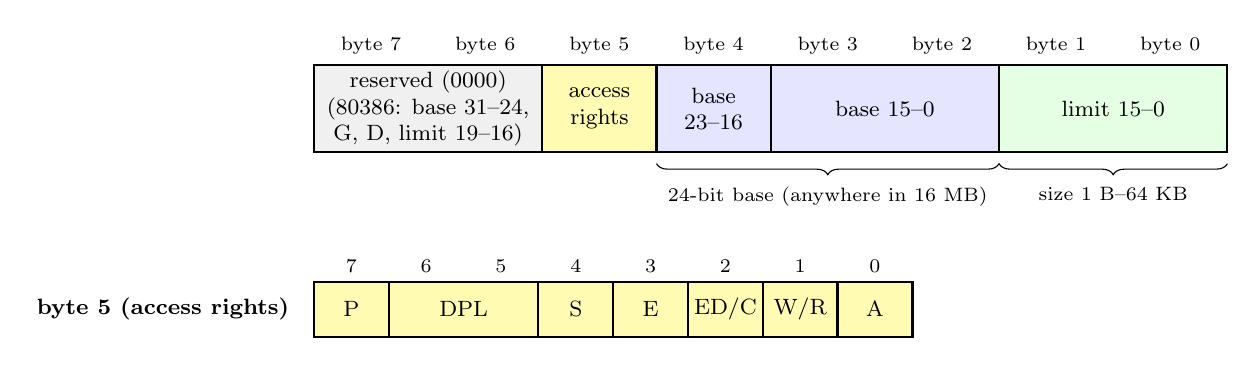
\begin{tikzpicture}[font=\small,x=1.45cm]
% bytes 7..0 left to right
\foreach \b in {0,...,7} \node[font=\scriptsize] at (7.5-\b,0.75) {byte \b};
\foreach \xa/\xb/\t/\c in {0/2/{reserved (0000)\\(80386: base 31--24,\\G, D, limit 19--16)}/gray!12,2/3/{access\\rights}/yellow!30,3/4/{base\\23--16}/blue!10,4/6/{base 15--0}/blue!10,6/8/{limit 15--0}/green!10} {
  \draw[thick,fill=\c] (\xa,-0.6) rectangle (\xb,0.5);
  \node[font=\footnotesize,align=center] at ({(\xa+\xb)/2},-0.05) {\t};
}
\draw[decorate,decoration={brace,mirror,amplitude=4pt}] (3,-0.75) -- (6,-0.75) node[midway,below=5pt,font=\scriptsize]{24-bit base (anywhere in 16 MB)};
\draw[decorate,decoration={brace,mirror,amplitude=4pt}] (6,-0.75) -- (8,-0.75) node[midway,below=5pt,font=\scriptsize]{size 1 B--64 KB};
% access rights byte expanded
\begin{scope}[yshift=-2.6cm,x=0.95cm]
\node[font=\footnotesize\bfseries,anchor=east] at (-0.2,0) {byte 5 (access rights)};
\foreach \i/\t/\w in {0/P/1,1/DPL/2,3/S/1,4/E/1,5/{ED/C}/1,6/{W/R}/1,7/A/1} {
  \draw[thick,fill=yellow!30] (\i,-0.35) rectangle (\i+\w,0.35);
  \node[font=\footnotesize] at (\i+\w/2,0) {\t};
}
\foreach \i/\b in {0/7,1/6,2/5,3/4,4/3,5/2,6/1,7/0} \node[font=\scriptsize] at (\i+0.5,0.55) {\b};
\end{scope}
\end{tikzpicture}
\end{document}
